%----------------------------------------------------------------------------
\chapter{Irodalomkutatás}
\label{sec:Search}
%----------------------------------------------------------------------------

\section{Felhasznált technológiák}
\label{sec:Technologies}

Ebben a fejezetben bemutatom az általam használt technológiákat amiket használtam és segítettek ennek a dolgozatnak a megírásában és elkészítésében.

\subsection{Jetpack Compose}

A Jetpack Compose a korábbi Android fejlesztési módszer mellett hozott létre egy alternatív megoldást.
Kezedtebn nem lehetett tudni, hogy a fejlesztők hogyan fognak reagálni az új irányra.
Korábban a Java nyelv mellett megjelent a Kotlin nyelv is, ami később szinte teljesen leváltotta az elődjét.
Ebből arra lehetett következtetni, hogy egy új és modernebb megoldás meg tudja állni a helyét az XML View megoldást ellenében.
Jelenleg mind a két megoldás támogatott, de a fejlsztések iránya egyértelműen a Compose felé húz.

"A Jetpack Compose egy új, deklaratív UI toolkit, amit a Google hozott létre kifejezetten natív Android alkalmazások fejlesztéséhez."\cite{GettingStartedWithJetpackCompose}
A deklaratív nyelvekhez hasonlóan, azt kellmegadnunk, hogy mit szeretnénk látni és nem azt leírni, hogy ez hogyan történjen meg.
Nekünk elegendő azt leírni, hogy a gomb hogyan nézzen ki és hol legyen és megadni egy lambda paraméternek, hogy a megnyomása soránmi történjen.
Mivel ez egy UI toolkit, ezért az összes vezerlő és szerkezeti elem hasonlóan néz ki, hasonlóan lehet használni így a fejlesztői és a felhasználói élmény is egységes és megszokott minőségű lesz minden alkalommal.
A Google ezt a Material design segítségével hozta létre, illetve annak újabb változataival. Erről részletesebben itt találhatók információk: \url{https://m3.material.io/}.

Az alábbiakban egy a Google által írt rövid kódrészleten bemutatom a legfontosabb részeit a Compose alapjainak.\cite{BasicCodelab}
Az első lépése az alaklamzás elkészítésének az a Composable függvény megírása.
Minden a UI-t megjelenítő függvény a @Composable annotációt viseli.
Innentől kezdve hagyományos Kotlin függvényként viselkedik, megadahatunk tetszőleges paramétereket (name, modifier) és alapértelmezett értékeket is.
Egy Composable függvényből tetszőleges másik Composable függvény meghívható megfelelőláthatóság esetén.
Ilyen például a Text() is ami a Material könyvtárnak egyik tagja és egyszerű szöveget jelenít meg.

A UI megírása után ezt a megfelelő helyen meg is kell jelenítenünk, erre az alkalmazás belépési pontja után van lehetőségünk.
Android esetén ez az activity onCreate függvénye.
A setContent vár egy lambda függvényt, aminek viselnie kell a @Composable annotációt, használhatjuk hozzá a Kotlin trailing lambda megoldását, aholis, ha az utolsó paramétere a függvénynek egy lambda, akkor a többi paraméter megadása után {} között megadhatjuk afüggvény törzsét.
A BasicsCodelabTheme is egy Composable függvény amiben az alap beállítások után meghívhatjuk a saját Greeting függvényünket.
A UI felépítse innentől kezdve már egyszerű.
A Composable függvények megírása után egymásból meghívva azokat előáll az alkalmazás.

\begin{lstlisting}
    @Composable
    fun Greeting(name: String, modifier: Modifier = Modifier) {
        Text(
            text = "Hello $name!",
            modifier = modifier
        )
    }

    class MainActivity : AppCompatActivity() {
        override fun onCreate(savedInstanceState: Bundle?) {
            super.onCreate(savedInstanceState)
            setContent {
                BasicsCodelabTheme {
                    // A surface container using the 'background' color from the theme
                    Surface(
                    modifier = Modifier.fillMaxSize(),
                    color = MaterialTheme.colorScheme.background
                    ) {
                        Greeting("Android")
                    }
                }
            }
        }
    }

    // Jetpack Compose forráskód
    public fun ComponentActivity.setContent(
        parent: CompositionContext? = null,
        content: @Composable () -> Unit
    )
\end{lstlisting}

A következőkben bemutatom a UI toolkit fontosabb általam használt részeit.
Kitérek arra, hogy mire jó, miért ezt használtam és hogyan lehet őket hatékonyan felhasználni a legújabb Compose Multiplatform verziókban.

\subsubsection{State és StateFlow}
A State és a StateFlow hasnló problémára ad megoldást.
A State alapvetően Compose sepcifikus megoldás, ha változik az értéke akkor a lefut a recomposoition.
Ezzel szemben a StateFlow a Kotlin nyelvben általánosan használt eszköz és sokkal bővebb felhasználással rendelkezik, mint az egyszerű State.
Az egyszerű Stateet általában egy Composable függvényen belül használják, míg a a StateFlowt ViewModelekben.
Ennek ellénére mind a két megoldás tökéletesen alkalmazható, jelenleg már Compose Multiplatform alkalmazásokban is.
Mivel ViewModelben használva az adatok nem besznek el a képernyő elforgatása során ezért egyszerűbb műveletekre és adaokra nincs lényegi különbség a működésben. 

"A StateFlow előnyei:"\cite{StateVsStateFlow}
\begin{itemize}
    \item \emph{"Flow operátorok:} A StateFlow támogat olyan operátorokat, mint a map, filter, és combine, lehetővé téve az adatok rugalmas feldolgozását és összetett adatfolyamok létrehozását."
    \item \emph{"Folyamat-megszakadás kezelése:} A SavedStateHandle-lel kombinálva biztosítja az UI állapot megőrzését, még a képernyő elforgatása vagy újraindítás esetén is."
    \item \emph{"ViewModel újrafelhasználhatóság:} A StateFlow lehetővé teszi a ViewModel függetlenítését a UI-rétegtől, ami elősegíti a moduláris, tesztelhető és újrafelhasználható architektúrát."
\end{itemize}

A lenti kódban láthatunk példát mind az egyszerű State használatára, ebben az esetben a Screen állapotát tárolom el Statekben.
A megjelnített adatok itt a StateFlow logikáját követik. 
Létezik egy privát MutableStateFlow amin történnek a változások például, ha adat érkezik.
Van egy másik azonos nevű érték is ami ugyan annak a StateFlownak egy immutábilis változata, ehhez fér hozzá a UI, így onnan nem érkezhet változás közvetlenül a StateFlowba.
Amennyiben erre szükség van, a viewmodel biztosíthat erre vonatkozóan függvényeket és beállíthatja a privát MutableStateFlow értékét.

\begin{lstlisting}
class TopicListViewModel: ViewModel() {
    var topicListScreenUiState: TopicListScreenUiState by mutableStateOf(TopicListScreenUiState.Loading)
    private val _topicListUiState = MutableStateFlow(TopicListUiState())
    val topicListUiState: StateFlow<TopicListUiState> = _topicListUiState
...
    fun getAllTopicList(){
        topicListScreenUiState = TopicListScreenUiState.Loading // State változtatása
        viewModelScope.launch {
            topicListScreenUiState = try{    // State változtatása
                val result = ApiService.getAllTopicNames()
                _topicListUiState.value = TopicListUiState(     //StateFlow változtatása
                    topicList = result.map { nameDto ->
                        TopicRowUiState(
                            topic = nameDto.name,
                            id = nameDto.uuid
                        )
                    }
                )
                TopicListScreenUiState.Success(result) // State változtatása
            } catch (e: IOException) {
                TopicListScreenUiState.Error.errorMessage = e.toString()// "Network error"
                TopicListScreenUiState.Error // State változtatása
            }
        }
    }
}
\end{lstlisting}

\subsubsection{ViewModel}
Az Android ViewModel már használható Kotlin- és Compose Multiplatform környezetekben is\cite{ViewModelKMP}, így természetesen ezt a jól bevált megoldást választottam.
Egy rövid összefoglalót szeretnék adni a hivatalos dokumentáció alapján a képességeiről:\cite{ViewModelAndroid}

A ViewModel az Android Jetpack része, és az UI állapotának megőrzésére szolgál konfigurációs változások során, például képernyőforgatáskor. \refstruc{fig:ViewModel} Fő előnyei közé tartozik az állapot tartósítása és az üzleti logika elérése a UI-rétegben. A ViewModel segít elválasztani az adatkezelést a UI-rétegtől, ehhez a ViewModelben felhasználható a Kotlin coroutine ami egyfajta aszinkron működést tesz lehetővé, és kompatibilis olyan Jetpack könyvtárakkal, mint a Hilt, Compose, és a Navigation. Best practice szerint kerülni kell az életciklushoz kötött objektumok tárolását benne, hogy elkerüljük a memóriaszivárgást. 

Mint minden MVM és MVVM architektúrában az adatok elérése, átalakítása a UI számára, tartós tárolása a ViewModel feladata.
Több megközelítés is lehetséges: minden képernyő kapjon egy saját ViewModelt; egy ViewModel tudjon többet és legyen újra felhasznáva több képernyőn.
Én az első megoldást választottam, így könnyebb kezeleni a különböző képrenyők állaptait és egyszerűbb átlátni egy-egy egységet.

\begin{figure}[!ht]
    \centering
    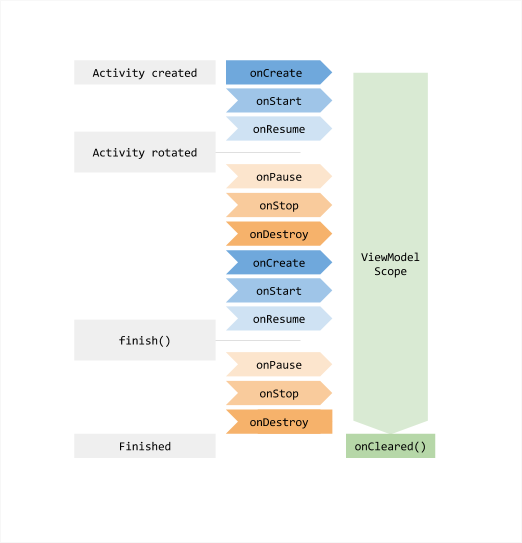
\includegraphics[width=150mm, keepaspectratio]{figures/viewmodel-lifecycle.png}
    \caption{A ViewModel álltalánosságban véve hosszabb életű, mint egy View. Ez különsöen igaz Android környezetben, ahol számolni kell a képernyő elforgatással és az alaklmazás háttérbe kerülésével. A tartósan tárolnikívánt adatokat ezért mindig ViewModel kell tárolni. \cite{ViewModelAndroid}}
    \label{fig:ViewModel}
\end{figure}

\subsubsection{Navigation and routing}

Az Androidban már jól műküdő navigációrt felelős könyvtárak már használhatóak a Kotlin Multiplatform fejlesztéséhez \cite{NavigationKMP}.
Ennk mindösszesen pár egyszerű lépése van, így könnyű használni és rugalamsan működik minden környezettel.
A következők a szükséges lépések: \cite{NavigationKMP}.
\begin{enumerate}
    \item "Sorold fel a navigációs gráfban szereplő útvonalakat, mindegyik egyedi string határozza meg az útvonalat."
    \item "Hozz létre egy NavHostController példányt a navigáció kezeléséhez"
    \item "Adj hozzá egy NavHost komponenst az alkalmazásodhoz:"
        \begin{itemize}
            \item "Válaszd ki a kezdő útvonalat a korábban definiált útvonalak közül."
            \item "Hozd létre a navigációs gráfot közvetlenül a NavHost részeként vagy programozottan a NavController.createGraph() függvénnyel."
        \end{itemize}
\end{enumerate}

\begin{lstlisting}

    //Első lépés: útvonalak létrehozása
//Érdemes sealed classt használni és data objectként létrehozni a routeokat
sealed class ExamDestination(val route: String) {
    //Lehet egyszerű
    data object LoginScreenDestination : ExamDestination("LoginScreen")

    //Vagy paraméterekkel és adatokkal ellátott
    data object TopicDetailsDestination : ExamDestination("TopicDetails") {
        const val topicIdArg = "0"
        val routeWithArgs = "$route/{$topicIdArg}"
    }
}

//Második lépés: NavController létrehozása
fun NavigationComponent() {
    MaterialTheme {
        val navController = rememberNavController() //Itt történik
        Scaffold() { innerPadding ->
            ExamNavHost(    //Paraméternek egy Composable függvényt vár, ezen belül is egy NavHost függvényt
                navController = navController,
                modifier = Modifier.padding(innerPadding)
            )
        }
    }
}

//Harmadik lépés: NavHost komponens hozzáadása
actual fun ExamNavHost(
    navController: NavHostController,
    modifier: Modifier
) {
    NavHost(
        navController = navController,  //NavController hozzárendelése
        startDestination = ExamDestination.MainScreenDestination.route, //Kezdő útvonal beállítása
        modifier = modifier
    ) {
        //Navigácós gráf egy elemének létrehozása
        composable(
            route = ExamDestination.TopicListDestination.route,
        ) {
            TopicListScreen(
                addNewTopic = { navController.navigate(ExamDestination.NewTopicDestination.route) },
                navigateToTopicDetails = { topicId ->
                    navController.navigate("${ExamDestination.TopicDetailsDestination.route}/${topicId}")
                },
                navigateBack = { navController.popBackStack() }
            )
        }
    }
}
\end{lstlisting}

\section{KotlinX Serilizáció}

\section{Ktor}

\section{CameraX}

\subsection{ML-Kit}

\section{ACCOMPANIST-engedélykezelés}

\subsection{pdfbox és PdfDocument}

\section{Kotlin- és Compose Multiplatform}

\section{Gradle build rendszer}

\section{Fejlesztőkörnyeztek}

\section{REST API és adatbázis}

\section{Kipróbált, de végül nem használt egyéb érdekes megoldások}